\section{BindingDB}
BindingDB \cite{gilson2016bindingdb} is an accessible database of drug target interactions and measured binding affinity values. With statistics as of February 2021, it can be listed as follows: It contains 41.328 entries, 8.202 protein targets each with a DOI, and 2.114.159 binding data for 928.022 small molecules. There are 2,823 protein-ligand crystal structures with BindingDB binding affinity measures for proteins with 100\% sequence identity, and 8.263 crystal structures allowing 85\% sequence identity of proteins. 2.077.458 Ki (nM), Kd (nM), IC50 (nM), EC50 (nM) values were compiled from the database within the scope of the thesis. 

To benchmark the performance of graph-based representational learning we use BDB dataset \cite{ozccelik2021chemboost} that is extracted from the BindingDB database. 24.404 binding affinities observed for all pairs of 924 ligand and 480 proteins, measured by the $pK_d$ value (log transformed kinase dissociation constant). The number of ligands with strong binding affinity values is 3428 (i.e., $pK_d \geq 7$) according to literature \cite{he2017simboost}. Figure \ref{fig:bdb} illustrates the distribution of the binding affinity values of proteins - ligand pairs in BDB dataset. 

\begin{figure}
    \centering
        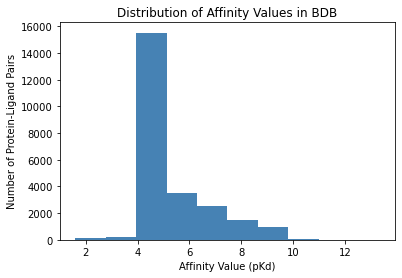
\includegraphics[width=0.5\linewidth]{chapters/datasetpreparation/figures/bdb.png} 
    \caption{Distribution of binding affinity values in BDB.}
    \label{fig:bdb}
\end{figure}

BDB dataset consists of 5 different setups for training and evaluating the model performance. To evaluate the performance of DeepDTA, we trained DeepDTA model with the knowledge derived from heterogeneous networks on five training setups of BDB dataset \cite{ozccelik2021chemboost}, and test the models in the corresponding test sets. 